\documentclass{article}

% if you need to pass options to natbib, use, e.g.:
\PassOptionsToPackage{numbers, compress}{natbib}
% before loading neurips_2026

% The authors should use one of these tracks.
% Before accepting by the NeurIPS conference, select one of the options below.
% 0. "default" for submission
% \usepackage{neurips_2026}
% the "default" option is equal to the "main" option, which is used for the Main Track with double-blind reviewing.
% 1. "main" option is used for the Main Track
%  \usepackage[main]{neurips_2026}
% 2. "position" option is used for the Position Paper Track
%  \usepackage[position]{neurips_2026}
% 3. "eandd" option is used for the Evaluations & Datasets Track
 % \usepackage[eandd]{neurips_2026}
 % if you need to opt-in for a single-blind submission in the E&D track:
 %\usepackage[eandd, nonanonymous]{neurips_2026}
% 4. "creativeai" option is used for the Creative AI Track
%  \usepackage[creativeai]{neurips_2026}
% 5. "sglblindworkshop" option is used for the Workshop with single-blind reviewing
 % \usepackage[sglblindworkshop]{neurips_2026}
% 6. "dblblindworkshop" option is used for the Workshop with double-blind reviewing
%  \usepackage[dblblindworkshop]{neurips_2026}

% After being accepted, the authors should add "final" behind the track to compile a camera-ready version.
% 1. Main Track
%  \usepackage[main, final]{neurips_2026}
% 2. Position Paper Track
%  \usepackage[position, final]{neurips_2026}
% 3. Evaluations & Datasets Track
 % \usepackage[eandd, final]{neurips_2026}
% 4. Creative AI Track
%  \usepackage[creativeai, final]{neurips_2026}
% 5. Workshop with single-blind reviewing
%  \usepackage[sglblindworkshop, final]{neurips_2026}
% 6. Workshop with double-blind reviewing
%  \usepackage[dblblindworkshop, final]{neurips_2026}
% Note. For the workshop paper template, both \title{} and \workshoptitle{} are required, with the former indicating the paper title shown in the title and the latter indicating the workshop title displayed in the footnote.
% For workshops (5., 6.), the authors should add the name of the workshop, "\workshoptitle" command is used to set the workshop title.
% \workshoptitle{WORKSHOP TITLE}

% "preprint" option is used for arXiv or other preprint submissions
\usepackage[preprint]{neurips_2026}

% to avoid loading the natbib package, add option nonatbib:
%    \usepackage[nonatbib]{neurips_2026}

\usepackage[utf8]{inputenc} % allow utf-8 input
\usepackage[T1]{fontenc}    % use 8-bit T1 fonts
\usepackage{hyperref}       % hyperlinks
\usepackage{url}            % simple URL typesetting
\usepackage{booktabs}       % professional-quality tables
\usepackage{amsfonts}       % blackboard math symbols
\usepackage{nicefrac}       % compact symbols for 1/2, etc.
\usepackage{microtype}      % microtypography
\usepackage{xcolor}         % colors

% Note. For the workshop paper template, both \title{} and \workshoptitle{} are required, with the former indicating the paper title shown in the title and the latter indicating the workshop title displayed in the footnote. 
\title{Trust Region Policy Distillation}


% The \author macro works with any number of authors. There are two commands
% used to separate the names and addresses of multiple authors: \And and \AND.
%
% Using \And between authors leaves it to LaTeX to determine where to break the
% lines. Using \AND forces a line break at that point. So, if LaTeX puts 3 of 4
% authors names on the first line, and the last on the second line, try using
% \AND instead of \And before the third author name.

% new
\usepackage{amsmath}
\usepackage{amssymb}
\usepackage{mathtools}
\usepackage{amsthm}
\usepackage{graphicx}
\usepackage{colortbl}
\usepackage{array}
\usepackage{wrapfig}
\usepackage{algorithm}
\usepackage{algorithmic}
\usepackage{multirow}

%%%%%%%%%%%%%%%%%%%%%%%%%%%%%%%%
% THEOREMS
%%%%%%%%%%%%%%%%%%%%%%%%%%%%%%%%
\theoremstyle{plain}
\newtheorem{theorem}{Theorem}[section]
\newtheorem{proposition}[theorem]{Proposition}
\newtheorem{lemma}[theorem]{Lemma}
\newtheorem{corollary}[theorem]{Corollary}
\theoremstyle{definition}
\newtheorem{definition}[theorem]{Definition}
\newtheorem{assumption}[theorem]{Assumption}
\theoremstyle{remark}
\newtheorem{remark}[theorem]{Remark}

\graphicspath{{figures/}}

\definecolor{0}{gray}{0.96}
\definecolor{1}{HTML}{F9F7ED}
\definecolor{2}{HTML}{f98e71}

\hypersetup{
	colorlinks=true, % 将链接的边框（丑陋的方框）替换为彩色文本
	linkcolor=2,     % 内部链接的颜色（如公式引用、图表引用、Section跳转）
	citecolor=2,     % 文献引用的颜色（如 [1], [2]）
	urlcolor=black,  % 外部 URL 链接的颜色
	filecolor=black  % 本地文件链接的颜色
}


%\author{%
%  Zhengpeng Xie\\
%  \texttt{zhengpengxie00@gmail.com} \\
%  \And
%  Li Lyna Zhang \\
%  \texttt{li.zhang@xingyunzhili.com} \\
%  \And
%  Zeke Xie \\
%  \texttt{zekexie@hkust-gz.edu.cn} \\
%  \And
%  Mao Yang \\
%  \texttt{maoyang@microsoft.com} \\
%}

\author{
	Zhengpeng Xie\thanks{Work done during an internship. $^{\dagger}$Project leader. $^{\ddagger}$Corresponding author.}$^{*}$ \qquad
	Li Lyna Zhang$^{\dagger}$ \qquad
	Zeke Xie$^{\ddagger}$ \qquad
	Mao Yang\\
	\texttt{zhengpengxie00@gmail.com} \qquad
	\texttt{li.zhang@xingyunzhili.com}\\
	\texttt{zekexie@hkust-gz.edu.cn} \qquad
	\texttt{maoyang@microsoft.com}
}


\begin{document}


\maketitle

\begin{figure*}[!h]
	\centering
	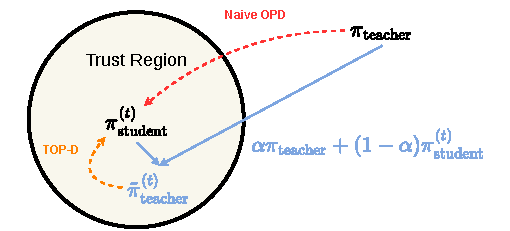
\includegraphics[scale=1.2]{teaser.pdf}
	\caption{While standard OPD forces direct teacher supervision and suffers from unstable optimization, TOP-D ensures stable training by dynamically constructing a proximal teacher at every iteration.}
	\label{teaser}
\end{figure*}



\begin{abstract}
	Big goals are hard to achieve all at once; breaking them into small steps is wiser. We present Trust Region Policy Distillation (TOP-D), which transforms the notoriously unstable, high-variance On-Policy Distillation (OPD) into a stable training paradigm by dynamically constructing a \textit{proximal teacher}. Theoretically, we establish a rigorous framework demonstrating that TOP-D inherently controls gradient variance. By providing a formal global convergence analysis alongside a monotonic improvement bound, we mathematically formalize the reliability and stability of the overall training dynamics. Empirically, TOP-D dramatically enhances training stability, sample efficiency, and final performance on mathematical reasoning tasks. More importantly, TOP-D introduces zero additional computational overhead, positioning itself as a promising alternative to the well-established OPD paradigm.
\end{abstract}



\begin{figure*}[!h]
	\centering
	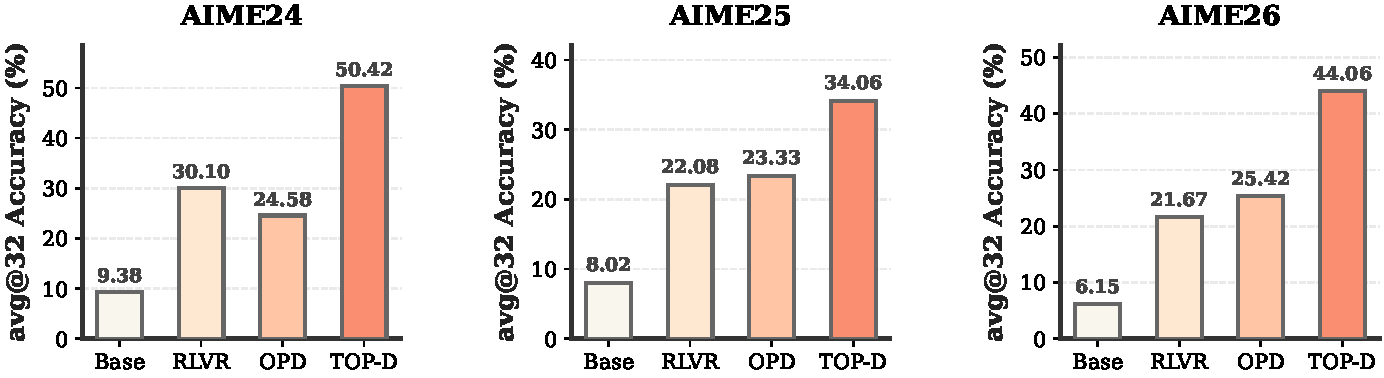
\includegraphics[scale=0.5]{aime_performance.pdf}
	\caption{The avg@32 accuracy on several AIME benchmarks for RLVR applied to the Qwen3-8B-Base model, and for OPD and TOP-D using Qwen3-30B-A3B-Instruct-2507 as the teacher model.}
\end{figure*}











\section{Introduction}
On-Policy Distillation (OPD) \citep{lu2025onpolicydistillation} has rapidly emerged as the prevailing paradigm for post-training Large Language Models (LLMs) \citep{yang2025qwen3, xiao2026mimo, zeng2026glm, yang2026nemotron, deepseekai2026deepseekv4}, in which the student learns from token-level signals provided by an external teacher. Mathematically, this is equivalent to reinforcement learning where the immediate reward is defined by the logarithmic probability ratio between the teacher and student policies. Consequently, the on-policy nature of OPD prevents the catastrophic forgetting of Supervised Fine-Tuning (SFT) \citep{shenfeld2026self}, while its dense rewards overcome the sample inefficiency and instability of Reinforcement Learning with Verifiable Rewards (RLVR) (as summarized in Table \ref{comparison of different paradigms}).

Despite its theoretical appeal, standard OPD suffers from severe optimization fragility in practice. The fundamental bottleneck of OPD lies in the inherent capacity gap between the target teacher and the student \citep{jang2026stable}. Because the standard distillation objective is driven by the logarithmic probability ratio between the two policies, the optimization dynamics are highly vulnerable to teacher-student disagreements. Recent studies have devoted considerable engineering efforts to mitigate this instability through various techniques, including teacher-student mixed sampling \citep{gu2024minillm}, reward clipping \citep{ko2026scaling}, top-$p$ sampling \citep{fu2026revisiting}, off-policy cold starts \citep{li2026rethinking}, and scaling to full-vocabulary supervision \citep{deepseekai2026deepseekv4}. However, these mitigation strategies remain largely empirical heuristics that fail to capture the underlying mechanism of the instability: the unbounded logarithmic probability difference between the teacher and student. Furthermore, these empirical methods inherently lack theoretical guarantees for reliable optimization.

In this paper, we present Trust Region Policy Distillation (TOP-D) to systematically resolve the inherent optimization instability of standard OPD. Specifically, to overcome the unbounded logarithmic signals, we dynamically construct an \textit{external proximal teacher} (as illustrated in Figure \ref{teaser} and Section \ref{External Proximal Teacher}) by interpolating the probability distributions of the target teacher and the current student. This mathematical construction transforms the unbounded distillation reward into a smooth, strictly lower-bounded signal, analytically preventing variance explosion. Building upon this stabilized objective, we further incorporate \textit{internal trust region iterations} (described in Section \ref{Internal Trust Region Iterations}) to better approximate the current proximal teacher, while simultaneously improving overall sample efficiency.

Crucially, while the proximal teacher is constructed conceptually, the practical objective mathematically reduces to a simple \textit{algebraic transformation} of the standard token-level OPD reward. As a result, TOP-D introduces zero additional computational overhead, serving as a plug-and-play module that is natively compatible with both state-of-the-art distributed training infrastructures \citep{shoeybi2019megatron, zhao2023pytorch} and high-throughput inference engines \citep{kwon2023efficient, zheng2024sglang}. Beyond this empirical elegance, our proposed framework establishes a rigorous theoretical closed-loop: while the external proximal teacher strictly bounds the gradient variance (described in Section \ref{Bounded Variance}), the internal trust region iterations guarantee monotonic policy improvement (described in Section \ref{Monotonic Improvement}), systematically minimizing the single-step optimization error to tightly close the overall asymptotic convergence gap (described in Section \ref{Convergence Analysis}).

In summary, the main contributions of this paper are as follows:
\begin{itemize}
	\item We propose TOP-D, a plug-and-play distillation paradigm that smooths the unbounded reward signal and safely breaks the strict on-policy data-reuse barrier of standard OPD.
	\item We establish a rigorous theoretical framework where the proximal teacher inherently bounds gradient variance to stabilize training, while our convergence analysis and monotonic improvement bound form a closed-loop to systematically minimize the asymptotic error.
	\item We empirically demonstrate that TOP-D dramatically improves reasoning capabilities on mathematical reasoning tasks, delivering a 25.84\% absolute improvement in avg@32 accuracy over standard OPD on AIME24 and consistently dominating RLVR and OPD baselines.
\end{itemize}




\begin{table}[!t]
	\centering
	\renewcommand{\arraystretch}{1.2}
	\resizebox{\linewidth}{!}{
		\begin{tabular}{c c c c c}
			\toprule
			Method & Sampling & Reward Signal & Training Stability & Theoretical Guarantee \\
			\midrule
			
			Supervised Fine-Tuning 
			& off-policy & \textbf{dense} & \textbf{high} & weak \\
			
			\rowcolor{1}
			Reinforcement Learning with Verifiable Rewards
			& \textbf{on-policy} & sparse & low & weak \\
			
			On-Policy Distillation
			& \textbf{on-policy} & \textbf{dense} & low & weak \\
			
			\rowcolor{1}
			Trust Region Policy Distillation 
			& \textbf{on-policy} & \textbf{dense} & \textbf{high} & \textbf{strong} \\
			
			\bottomrule
		\end{tabular}
	}
	\caption{Comparison of different paradigms.}
	\label{comparison of different paradigms}
\end{table}




\section{Preliminaries}
\subsection{On-Policy Distillation}\label{On-Policy Distillation}
Suppose we have an autoregressive language model $\pi_{\theta}$, where $\theta\in\Theta$ denotes the parameters. Given a prompt $x\sim\mathcal{D}_x$, the model generates response $y=(y_0,y_1,\dots,y_T)$\footnote{Here, $y_0$ denotes the special initial token and is not counted toward the response length.} autoregressively, where $T=\lvert y\rvert$ is the response length. Formally,
\begin{equation}
	\log\pi_{\theta}(y\mid x)=\sum_{t=1}^{\lvert y\rvert}\log\pi_{\theta}(y_t\mid x,y_{<t}),
\end{equation}
where $y_{<t}$ denotes $(y_0,y_1,\dots,y_{t-1})$. In the context of OPD, we aim to minimize the following \textit{reverse} KL divergence:
\begin{equation}\label{objective}
	\begin{split}
		\theta^*=\arg\min_{\theta}\mathcal{L}(\theta)&=\arg\min_{\theta}\mathbb{E}_{x\sim\mathcal{D}_x}\left[\mathcal{D}_{\mathrm{KL}}(\pi_{\theta}(\cdot\mid x),\pi^*(\cdot\mid x))\right]\\
		&=\arg\max_{\theta}\mathbb{E}_{x\sim\mathcal{D}_x,y\sim\pi_{\theta}(\cdot\mid x)}\left[\log\frac{\pi^*(y\mid x)}{\pi_{\theta}(y\mid x)}\right]=\arg\max_{\theta}J(\theta),\\
	\end{split}
\end{equation}
where $\pi^*$ is typically a stronger model. We are now ready to present the standard \textit{policy gradient} form of the objective \eqref{objective}:
\begin{equation}\label{policy gradient}
	\nabla_{\theta}J(\theta)=\mathbb{E}_{x\sim\mathcal{D}_x,y\sim\pi_{\theta}(\cdot\mid x)}\left[\sum_{t=1}^{\lvert y\rvert}\nabla_{\theta}\log\pi_{\theta}(y_t\mid x,y_{<t})\cdot\left(\sum_{k=t}^{\lvert y\rvert}\log\rho_k\right)\right],
\end{equation}
where $\rho_k=\frac{\pi^*(y_k\mid x,y_{<k})}{\pi_{\theta}(y_k\mid x,y_{<k})}$. In other words, we can treat $\log\rho_k$ as the immediate reward for the $k$-th token, i.e., $r_k=\log\rho_k$. However, the cumulative reward $\sum_{k=t}^{\lvert y\rvert}r_k$ introduces an inherent length bias as well as high variance. In practice, a common approach is to use the immediate reward $r_k$ directly.



\subsection{Reinforcement Learning Formulation}\label{Reinforcement Learning Formulation}
To establish a rigorous theoretical foundation, we cast autoregressive language modeling as a deterministic Markov Decision Process (MDP) defined by the tuple $\left(\mathcal{S},\mathcal{A},\mathcal{P},r,\mu_0\right)$.
\begin{itemize}
	\item \textbf{State space $\mathcal{S}$ and action space $\mathcal{A}$.} State $s_t = (x, y_{<t})$ represents the prompt and prefix. The action space $\mathcal{A} = \mathcal{V} $ includes the vocabulary and the \texttt{EOS} token. To rigorously handle variable-length sequences, we augment $\mathcal{S}$ with a permanent \textit{absorbing state} $s_\bot$.
	\item \textbf{Dynamics $\mathcal{P}$ and initial distribution $\mu_0$.} The initial state distribution $\mu_0(s)$ follows the prompt distribution $\mathcal{D}_x$ and the special initial token $y_0$. Transitions are \textit{deterministic}: selecting $a \neq \texttt{EOS}$ appends $a$ to the prefix, while selecting $\texttt{EOS}$ definitively transitions to $s_\bot$.
	\item \textbf{Reward function $r$.} The immediate reward is the distillation signal: $r(s, a) = \log \frac{\pi^*(a \mid s)}{\pi(a \mid s)}$. To prevent infinite accumulation after termination\footnote{Assume that $\pi(\texttt{EOS}\mid s_\bot)=1$.}, we set $r(s_\bot, a) \equiv 0$ for any $a\in\mathcal{A}$.
\end{itemize}

Let $\pi: \mathcal{S} \to \Delta(\mathcal{A})$ be a stochastic policy. Operating in the undiscounted setting ($\gamma=1$), the action value function $Q^\pi(s, a)$ is defined as $Q^\pi(s, a) = \mathbb{E}_{\pi} \left[ \sum_{k=0}^{\infty} r(s_{t+k}, a_{t+k})\mid s_t=s, a_t=a \right]$. The state value function $V^\pi(s)$ is strictly obtained by marginalizing $Q^\pi$ over the policy: $V^\pi(s) = \mathbb{E}_{a \sim \pi(\cdot \mid s)} \left[ Q^\pi(s, a) \right]$. Consequently, we define the advantage function, which forms the basis for policy improvement bounds, as $A^\pi(s, a) = Q^\pi(s, a) - V^\pi(s)$. To decouple sequential dependencies, we introduce the \textit{unnormalized} state distribution $d^\pi(s) = \sum_{t=1}^{\infty}\mathbb{P}(s_t = s \mid \pi)$. The true objective of a policy $\pi$ is the expected cumulative reward over the infinite horizon:
\begin{equation}\label{original eta}
	\eta(\pi) = \mathbb{E}_{x \sim \mathcal{D}_x, y \sim \pi(\cdot \mid x)} \left[ \sum_{t=1}^{\infty} r(s_t, a_t) \right].
\end{equation}

While this abstract MDP formalization is adopted for the theoretical proofs in Section \ref{Monotonic Improvement}, the remainder of the paper defaults to the notation established in Section \ref{On-Policy Distillation}.














\section{Methodology}
This section details the design of our core algorithm, Trust Region Policy Distillation (TOP-D). We begin in Section \ref{External Proximal Teacher} by constructing a \textit{proximal teacher} to stabilize training. Subsequently, in Section \ref{Internal Trust Region Iterations}, the current student approximates this proximal teacher by performing \textit{trust region iterations}. Finally, Section \ref{Trust Region Policy Distillation} outlines the practical implementation of the TOP-D algorithm.

\subsection{External Proximal Teacher}\label{External Proximal Teacher}
The fundamental challenge in standard On-Policy Distillation (OPD) arises from the inherent capacity gap between the student policy $\pi_{\theta}$ and the target teacher policy $\pi^*$. As defined in Equation \eqref{policy gradient}, the optimization dynamics heavily rely on the probability ratio $\rho_k=\frac{\pi^*(y_k\mid x,y_{<k})}{\pi_{\theta}(y_k\mid x,y_{<k})}$. In extreme cases where the teacher assigns a near-zero probability to a generated token ($\pi^*\rightarrow0$), the immediate reward $r_k=\log\rho_k$ diverges to negative infinity. This unbounded penalty destabilizes the policy gradient, making the optimization process extremely fragile.

\begin{wrapfigure}{r}{0.38\textwidth}
	\centering
	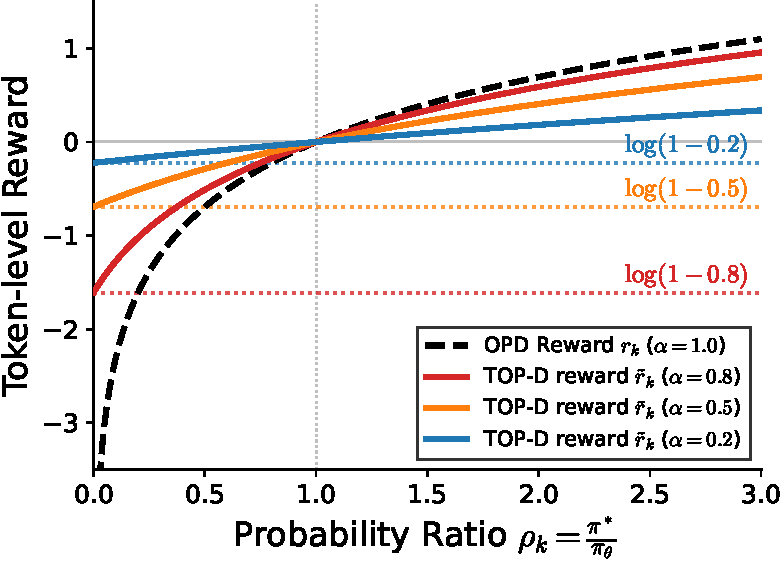
\includegraphics[width=0.35\textwidth]{reward_comparison.pdf}
	\caption{Reward curves of $r_k$ and $\tilde{r}_k$.}
	\label{reward comparison}
\end{wrapfigure}

To address this instability, we draw inspiration from \textit{trust region} methods in reinforcement learning \citep{schulman2015trust, schulman2017proximal, xie2025simple}, which restrict policy updates from taking destructively large steps. Rather than forcing the student to perfectly imitate a rigid teacher, we dynamically construct an intermediate, localized target distribution. We term this surrogate target the \textit{proximal teacher} $\tilde{\pi}^*$. Formally,
\begin{equation*}
	\tilde{\pi}^*(y_k\mid x,y_{<k})=\alpha\pi^*(y_k\mid x,y_{<k})+(1-\alpha)\pi_{\theta}(y_k\mid x,y_{<k}),
\end{equation*}
where $\alpha\in(0,1)$ is the coefficient that controls the interpolation strength. In fact, the proximal teacher inherently smooths the token-level reward $r_k$. Specifically,
\begin{equation}
	\tilde{r}_k=\log\frac{\tilde{\pi}^*(y_k\mid x,y_{<k})}{\pi_{\theta}(y_k\mid x,y_{<k})}=\log\left(\alpha\frac{\pi^*(y_k\mid x,y_{<k})}{\pi_{\theta}(y_k\mid x,y_{<k})}+1-\alpha\right)=\log\left(\alpha\rho_k+1-\alpha\right).
\end{equation}
When $\alpha=1$, it reduces to the original OPD reward $r_k$. Thanks to mathematics, we do not need to explicitly construct a proximal teacher to obtain the new reward $\tilde{r}_k$. Figure \ref{reward comparison} visualizes the OPD reward $r_k$ and our proposed reward $\tilde{r}_k$ with respect to the probability ratio $\rho_k$. We can see that $\tilde{r}_k$ is strictly bounded from below\footnote{$\log(\alpha x+1-\alpha)\geq\log(1-\alpha)$ when $x\in(0,+\infty)$ and $\alpha\in(0,1)$.} as $\rho_k\rightarrow0$. Moreover, we explicitly justify our choice of interpolating in the \textit{probability space} instead of the \textit{log-probability space} to construct the proximal teacher, since setting $\log\tilde{\pi}^*(y_k\mid x,y_{<k})=\alpha\log\pi^*(y_k\mid x,y_{<k})+(1-\alpha)\log\pi_{\theta}(y_k\mid x,y_{<k})$ yields
\begin{equation}
	\tilde{r}_k=\alpha r_k,
\end{equation}
which is merely a naive scaling of the original OPD reward.



\subsection{Internal Trust Region Iterations}\label{Internal Trust Region Iterations}
With the proximal teacher established, the student policy is optimized to maximize the expected cumulative reward $\tilde{R}_t=\sum_{k=t}^{\lvert y\rvert}\tilde{r}_k$. While standard OPD relies on continuous online sampling, it fundamentally operates in a strictly on-policy manner. In the naive formulation, once the student policy is updated, the previously generated trajectories are immediately discarded. This results in notoriously low sample efficiency, lacking the capacity to reuse data.

Inspired by modern trust region algorithms \citep{schulman2015trust, schulman2017proximal, xie2025simple}, we analogously decouple the \textit{behavior policy} $\pi_{\theta_{\mathrm{old}}}$ and the \textit{target policy} $\pi_{\theta}$ to inherit their high sample efficiency. Specifically,
\begin{equation}
	J(\theta)=\mathop{\mathbb{E}}_{\substack{x\sim\mathcal{D}_x\\\{y^{i}\}_{i=1}^{G}\sim\pi_{\theta_{\mathrm{old}}}(\cdot\mid x)}}\left[\frac{1}{\sum_{i=1}^{G}\lvert y^{i}\rvert}\sum_{i=1}^{G}\sum_{t=1}^{\lvert y^{i}\rvert}\left\{\min\left[p_t^i\cdot\hat{A}_t^i,\mathrm{clip}\left(p_t^i,1-\epsilon,1+\epsilon\right)\cdot\hat{A}_t^i\right]\right\}\right].
\end{equation}
Here, we follow the group-based reinforcement learning settings \citep{shao2024deepseekmath, guo2025deepseek}, where the superscript $i$ indexes different model responses. $p_t^i=\frac{\pi_{\theta}(y_t^i\mid x,y_{<t}^i)}{\pi_{\theta_{\mathrm{old}}}(y_t^i\mid x,y_{<t}^i)}$ is the importance sampling ratio. We adopt a more fine-grained token-level normalized advantage $\hat{A}_t^i$ to better exploit dense reward signals, as illustrated in Figure \ref{advantage}. For each prompt, the advantage relies on a token-level reward $\tilde{R}_t$, which combines the immediate reward and a length-normalized future return \citep{gu2024minillm}, i.e.,
\begin{equation}
	\tilde{R}_k^i=\tilde{r}_k^i+\frac{1}{\lvert y^i\rvert-k}\sum_{j=k+1}^{\lvert y^i\rvert}\tilde{r}_j^i.
\end{equation}
We empirically observe that this prevents the model from generating overly short or excessively long responses. The mean $\mu$ and standard deviation $\sigma$ within each group are calculated via $\mu=\mathrm{mean}\{\tilde{R}_k^i\}$ and $\sigma=\mathrm{std}\{\tilde{R}_k^i\}$, where $i=1,\dots,G$ and $k=1,\dots,\lvert y^i\rvert$.

\begin{figure*}[!t]
	\centering
	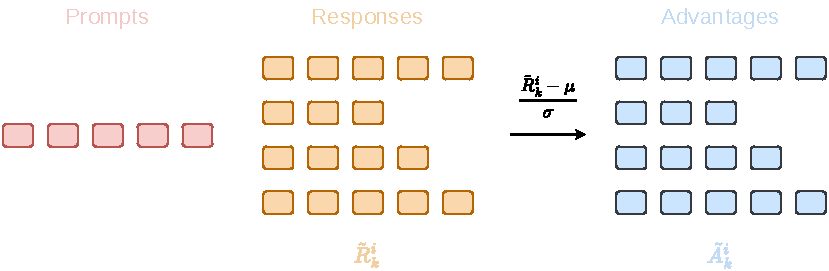
\includegraphics[scale=0.7]{adv.pdf}
	\caption{In contrast to \textit{sequence-level} advantage normalization, we perform \textit{token-level} normalization across the responses generated for a given prompt to better leverage the dense reward signal.}
	\label{advantage}
\end{figure*}




\subsection{Trust Region Policy Distillation}\label{Trust Region Policy Distillation}
In this section, we synthesize the concepts of the \textit{external proximal teacher} in Section \ref{External Proximal Teacher} and the \textit{internal trust region iterations} in Section \ref{Internal Trust Region Iterations} to formulate our complete algorithmic framework, Trust Region Policy Distillation (TOP-D), summarized in Algorithm \ref{topd}.

Standard OPD suffers from two fundamental bottlenecks: optimization fragility and low sample efficiency. TOP-D systematically resolves both through a unified design. First, the \textit{external proximal teacher} transforms the unbounded OPD reward into a smooth, lower-bounded reward $\tilde{r}_k$, intrinsically stabilizing the optimization process. Built upon this principle, the \textit{internal trust region iterations} decouple the behavior and target policies, breaking the strict on-policy data-reuse barrier. Crucially, these mechanisms are not merely empirical heuristics but share deep theoretical synergy. We rigorously formalize this framework and establish its mathematical guarantees in the Section \ref{Theoretical Analysis}.

\begin{algorithm}[!t]
	\caption{Trust Region Policy Distillation (TOP-D)}
	\label{topd}
	\begin{algorithmic}[1]
		\REQUIRE Student $\pi_{\theta}$, teacher $\pi^*$, dataset $\mathcal{D}_x$, interpolation $\alpha$, group size $G$, internal epochs $E$
		\WHILE{not converged}
		\STATE Initialize $\pi_{\theta_{\mathrm{old}}} \leftarrow \pi_{\theta}$
		\STATE Sample a batch of prompts $\mathcal{X}\subset\mathcal{D}_x$
		\FOR{each prompt $x\in\mathcal{X}$}
		\STATE Perform rollout to sample $G$ responses $\{y^{i}\}_{i=1}^{G}\sim\pi_{\theta_{\mathrm{old}}}(\cdot\mid x)$
		\STATE Compute TOP-D rewards $\tilde{r}_k^i\leftarrow\log\left(\alpha\frac{\pi^*(y_k^i\mid x,y_{<k}^i)}{\pi_{\theta_{\mathrm{old}}}(y_k^i\mid x,y_{<k}^i)}+1-\alpha\right)$
		\STATE Compute token-level returns $\tilde{R}_k^i\leftarrow\tilde{r}_k^i+\frac{1}{\lvert y^i\rvert-k}\sum_{j=k+1}^{\lvert y^i\rvert}\tilde{r}_j^i$
		\STATE Compute token-level advantages $\hat{A}_k^i\leftarrow\frac{\tilde{R}_k^i-\mu}{\sigma}$
		\ENDFOR
		\FOR{epoch $e = 1$ to $E$}
		\STATE $J(\theta)\leftarrow\frac{1}{\sum_{i=1}^{G}\lvert y^{i}\rvert}\sum_{i=1}^{G}\sum_{t=1}^{\lvert y^{i}\rvert}\left\{\min\left[p_t^i\cdot\hat{A}_t^i,\mathrm{clip}\left(p_t^i,1-\epsilon,1+\epsilon\right)\cdot\hat{A}_t^i\right]\right\}$
		\STATE Update $\theta$ by maximizing $J(\theta)$ using an optimizer
		\ENDFOR
		\ENDWHILE
	\end{algorithmic}
\end{algorithm}









\section{Theoretical Analysis}\label{Theoretical Analysis}
In this section, we establish a rigorous theoretical foundation for TOP-D. We begin in Section \ref{Bounded Variance} by proving that the proximal teacher inherently bounds gradient variance to stabilize optimization. Building upon this, we derive a global convergence bound in Section \ref{Convergence Analysis} by abstracting the learning dynamics. Finally, to minimize the local error bottleneck identified in this convergence analysis, we establish the monotonic improvement guarantee for our internal trust region iterations in Section \ref{Monotonic Improvement}.



\subsection{Bounded Variance}\label{Bounded Variance}
To rigorously analyze the gradient stability, we restrict our discussion to the autoregressive generation environment over a finite vocabulary $\mathcal{V}$. In policy gradient methods, the variance of the gradient is typically dominated by its \textit{second moment}, i.e., $\mathrm{Var}\left[g\right]\leq\mathbb{E}\left[\lVert g\rVert^2\right]$. Thus, our theoretical analysis will primarily focus on establishing an absolute upper bound for the gradient's second moment.
\begin{assumption}\label{assumption 1}
	We assume that the gradient of the student policy's log-probability (the score function) is uniformly bounded. That is, there exists a constant $M>0$, such that for any prompt $x\sim\mathcal{D}_x$, generated response $y\sim\pi(\cdot\mid x)$, and $k$-th token $y_k$, we have
	\begin{equation}
		\lVert\nabla_{\theta}\log\pi_{\theta}(y_k\mid x,y_{<k})\rVert\leq M.
	\end{equation}
\end{assumption}
Let $g_k=\nabla_{\theta}\log\pi_{\theta}(y_k\mid x,y_{<k})\cdot r_k$ denote the token-level policy gradient estimator for standard OPD, and $\tilde{g}_k=\nabla_{\theta}\log\pi_{\theta}(y_k\mid x,y_{<k})\cdot\tilde{r}_k$ denote the gradient estimator for our proposed TOP-D.
\begin{theorem}\label{bounded variance}
	Under Assumption \ref{assumption 1}, for any interpolation coefficient $\alpha\in(0,1)$, the variance of the TOP-D gradient estimator $\tilde{g}_k$ does not diverge across the entire probability space. Instead, it is strictly bounded by a uniform absolute limit:
	\begin{equation}
		\mathrm{Var}(\tilde{g}_k)\leq M^2\lvert\mathcal{V}\rvert\max\left\{\left(\log(1-\alpha)\right)^2, C^*\alpha\right\},
	\end{equation}
	where $C^*$ is a universal mathematical constant, and $\lvert\mathcal{V}\rvert$ denotes the size of the vocabulary $\mathcal{V}$.
\end{theorem}
\begin{proof}
	See Appendix \ref{proof of bounded variance}.
\end{proof}
\begin{remark}
	TOP-D employs an asymmetric operator to stabilize training. For heavy penalizations, it introduces a hard safety bound, $(\log(1-\alpha))^2$, preventing catastrophic divergence; for high rewards, it applies a linear dampening scaled by $C^*\alpha$. This effectively designates $\alpha$ as a direct variance controller. As $\alpha \to 1^-$, TOP-D recovers standard OPD, with its upper bound diverging ($(\log(1-\alpha))^2 \to \infty$) to reflect OPD's unbounded variance. Conversely, as $\alpha \to 0^+$, the variance vanishes.
\end{remark}












\subsection{Convergence Analysis}\label{Convergence Analysis}
To rigorously analyze the convergence properties of TOP-D, we abstract the construction of the proximal teacher as an iterative operator mapping over the policy space. Let $\Pi$ denote the space of all valid policies. To quantify the divergence within this space, we introduce the expected $L_1$ distance between any two policies $\pi_i, \pi_j$ as $d(\pi_i, \pi_j) = \mathbb{E}_{x \sim \mathcal{D}_x} \left[ \lVert \pi_i(\cdot \mid x) - \pi_j(\cdot \mid x) \rVert_1 \right]$. Next, we formalize the iterative process through the \textit{proximal teacher operator} $\mathcal{T}:\Pi\to\Pi$, given by
\begin{equation}\label{proximal teacher operator}
	\mathcal{T}(\pi)=\alpha\pi^*+(1-\alpha)\pi,
\end{equation}
where $\alpha\in(0,1)$ is the interpolation coefficient, and $\pi^*$ is the target teacher. Building upon this metric space, we are now ready to establish the following convergence analysis:
\begin{theorem}\label{convergence}
	For any initial student policy $\pi_0\in\Pi$, consider the iterative update process $\pi_{k+1}=\mathcal{T}(\pi_k)+\epsilon_k$\footnote{With a slight abuse of notation, let $\lVert\epsilon_k\rVert_1=d(\pi_{k+1},\tilde{\pi}_k^*)$, where $\tilde{\pi}_k^*=\mathcal{T}(\pi_k)$ is the proximal teacher at the $k$-th step.}, where $\epsilon_k$ accounts for the practical optimization error (e.g., function approximation and optimization noise) at the $k$-th global step, where $k\geq0$. Then, the following bound holds:
	\begin{equation}
		d(\pi_{k+1},\pi^*)\leq(1-\alpha)^{k+1}d(\pi_0,\pi^*)+\sum_{i=0}^{k}(1-\alpha)^{k-i}\lVert\epsilon_i\rVert_1.
	\end{equation}
	Furthermore, assuming the optimization process eventually stabilizes such that the asymptotic error is bounded by $\limsup_{k\rightarrow \infty}\lVert\epsilon_{k}\rVert_1\leq \epsilon_{\infty}$, we have
	\begin{equation}
		\limsup_{k \rightarrow \infty} d(\pi_{k+1}, \pi^*) \leq \frac{\epsilon_{\infty}}{\alpha}.
	\end{equation}
\end{theorem}
\begin{proof}
	See Appendix \ref{proof of convergence}.
\end{proof}
\begin{remark}
	The bound presented in Theorem \ref{convergence} not only reveals an inherent \textit{error forgetting} mechanism that isolates early high-variance updates, but also highlights a fundamental theoretical \textit{trade-off}: the asymptotic convergence gap is strictly bounded by $\epsilon_\infty/\alpha$. This implies that to break through the precision ceiling without compromising stability (i.e., keeping $\alpha$ small), the only viable path is to strictly minimize the single-step optimization error $\lVert\epsilon_k\rVert_1$. This theoretical bottleneck motivates the necessity of introducing \textit{internal trust region iterations} in the subsequent section.
\end{remark}


\subsection{Monotonic Improvement}\label{Monotonic Improvement}
As revealed in Theorem \ref{convergence}, the fundamental theoretical bottleneck of the proximal teacher framework lies in the asymptotic convergence gap bounded by $\epsilon_\infty/\alpha$. To tightly close this gap without compromising optimization stability (i.e., avoiding excessively large $\alpha$), it is imperative to rigorously minimize the single-step optimization error $\lVert\epsilon_k\rVert_1$. TOP-D achieves this via internal trust region iterations. In this section, we establish the theoretical insight of this mechanism by proving monotonic policy improvement. For mathematical rigor, we follow the notation established in Section \ref{Reinforcement Learning Formulation}.
\begin{assumption}\label{assumption 2}
	Given the fixed context window constraints inherent to autoregressive language models, we assume that any valid policy $\pi \in \Pi$ generates the \texttt{EOS} token within a finite maximum horizon $T_{\max}$. Consequently, the response length strictly satisfies $\lvert y\rvert \leq T_{\max}$, so $\sum_{s\neq s_\bot}d^{\pi}(s)<\infty$.
\end{assumption}
In our undiscounted setting ($\gamma=1$), the unnormalized measure $d^\pi(s)$ diverges because the permanent absorbing state $s_\bot$ dominates as $t \to \infty$. To construct a valid probability distribution over the meaningful transient states, we explicitly exclude $s_\bot$ and normalize $d^\pi(s)$.
\begin{definition}\label{normalized state distribution}
	We formally define the \textit{expected response length} of a policy $\pi$ as $\ell_\pi = \mathbb{E}_{x \sim \mathcal{D}_x, y \sim \pi(\cdot \mid x)}\left[\lvert y\rvert\right]$. Excluding $s_\bot$, the sum of the state distribution precisely evaluates to this length. Thus, we define the normalized state visitation measure $d^\pi_{\mathrm{norm}}(s) = \frac{d^\pi(s)}{\ell_\pi},\enspace s \neq s_\bot$.
\end{definition}
\begin{remark}
	This normalized measure enables an equivalent reformulation of the \textit{Performance Difference Lemma} \citep{kakade2002approximately}, strictly decoupling the sequence length from the single-step generation quality.
\end{remark}
We can thus rewrite the original objective \eqref{original eta} as $\eta(\pi)=\ell_{\pi}\cdot\mathbb{E}_{s \sim d^{\pi}_{\mathrm{norm}}(\cdot), a \sim\pi(\cdot \mid s)} \left[r(s,a)\right]$, and we are now ready to present the main theoretical result of this section:
\begin{theorem}\label{performance lower bound}
	Given Assumption \ref{assumption 2} and Definition \ref{normalized state distribution}, for any two policies, $\tilde{\pi}$ and $\pi$, the following bound holds:
	\begin{equation}
		\eta(\tilde{\pi})\geq\zeta_\pi(\tilde{\pi}) - 2\xi T_{\max}\ell_\pi\mathbb{E}_{s \sim d^{\pi}_{\mathrm{norm}}(\cdot)}\left[\mathcal{D}_{\mathrm{TV}}(\tilde{\pi}(\cdot \mid s),\pi(\cdot \mid s))\right],
	\end{equation}
	where $\zeta_\pi(\tilde{\pi})=\eta(\pi) + \ell_\pi\mathbb{E}_{s \sim d^\pi_{\mathrm{norm}}(\cdot), a \sim \tilde{\pi}(\cdot \mid s)} \left[ A^\pi(s, a) \right]$, and $\xi=\max_{s}\lvert\mathbb{E}_{a\sim\tilde{\pi}(\cdot\mid s)}\left[A^\pi(s,a)\right]\rvert$.
\end{theorem}
\begin{proof}
	See Appendix \ref{proof of performance lower bound}.
\end{proof}
\begin{remark}
	Let $\mathcal{M}_{\pi}(\tilde{\pi})$ denote the lower bound established in Theorem \ref{performance lower bound}. By definition, $\eta(\pi)=\mathcal{M}_{\pi}(\pi)$. Therefore, any policy update that improves the lower bound guarantees monotonic improvement on the true objective, i.e., $\eta(\tilde{\pi}) - \eta(\pi) \geq \mathcal{M}_\pi(\tilde{\pi}) - \mathcal{M}_\pi(\pi)$.
\end{remark}
As a result, optimizing $\mathcal{M}_{\pi}(\tilde{\pi})$ ensures that the original reverse KL divergence objective monotonically improves during the internal updates. Let the superscript $(n)$ denote the $n$-th step of the internal trust region iterations at the $k$-th global step, and let $\tilde{\pi}_k^* = \mathcal{T}(\pi_k)$ be the fixed proximal teacher. By iteratively optimizing $\mathcal{M}_{\pi}(\tilde{\pi})$, we obtain a monotonically decreasing sequence of KL divergences:
\begin{equation}
	\mathbb{E}_{x\sim\mathcal{D}_x}\left[\mathcal{D}_{\mathrm{KL}}^{(0)}\right]\geq\mathbb{E}_{x\sim\mathcal{D}_x}\left[\mathcal{D}_{\mathrm{KL}}^{(1)}\right]\geq\cdots\geq\mathbb{E}_{x\sim\mathcal{D}_x}\left[\mathcal{D}_{\mathrm{KL}}^{(n)}\right],
\end{equation}
where $\mathcal{D}_{\mathrm{KL}}^{(j)} \triangleq \mathcal{D}_{\mathrm{KL}}(\pi_k^{(j)}(\cdot \mid x),\tilde{\pi}_k^*(\cdot \mid x))$ denotes the reverse KL divergence objective at the $j$-th internal iteration. If the internal trust region optimization proceeds until the final expected divergence satisfies $\mathbb{E}_{x \sim \mathcal{D}_x}\left[\mathcal{D}_{\mathrm{KL}}^{(n)}\right] \leq \frac{1}{2}\delta^2$ where $\delta>0$, then by applying Pinsker's inequality $\lVert\epsilon_{k}\rVert_1=d(\pi_{k+1},\tilde{\pi}_k^*)=d(\pi_k^{(n)}, \tilde{\pi}_k^*)\leq\mathbb{E}_{x \sim \mathcal{D}_x}\left[\sqrt{2\mathcal{D}_{\mathrm{KL}}^{(n)}}\right]\leq\sqrt{2\mathbb{E}_{x\sim\mathcal{D}_x}\left[\mathcal{D}_{\mathrm{KL}}^{(n)}\right]}\leq\delta$ alongside Jensen's inequality, we rigorously guarantee that the optimization error satisfies $\lVert\epsilon_k\rVert_1\leq\delta$. This perfectly closes the overall theoretical loop: the internal trust region iterations mathematically guarantee the continuous minimization of the single-step optimization error $\epsilon_k$, thereby enabling the algorithm to tightly close the asymptotic convergence gap $\epsilon_\infty/\alpha$ defined in Theorem \ref{convergence}.




\section{Experiments}
In this section, we empirically validate the effectiveness of TOP-D. Specifically, Section \ref{Experimental Setup} details our validation datasets, model configurations, baseline methods, and implementation hyperparameters. Section \ref{Main Results} presents a comprehensive comparison of TOP-D against existing post-training baselines. Finally, Section \ref{Ablation Study} provides an in-depth analysis of the core components of our method, including the external proximal teacher and the internal trust region iterations, as well as the sensitivity analysis.

\subsection{Experimental Setup}\label{Experimental Setup}
\textbf{Datasets and benchmarks.} We conduct our training phase using the DAPO-Math-17k \citep{yu2025dapo} dataset, a high-quality mathematical reasoning corpus. For validation, we benchmark the post-trained models on widely recognized and challenging mathematical reasoning competitions like AIME and AMC.

\textbf{Models and baselines.} To comprehensively investigate the scalability of TOP-D and its robustness across different teacher-student capacity gaps, we employ two distinct base models as students: Qwen3-1.7B-Base \citep{yang2025qwen3} and Qwen3-8B-Base \citep{yang2025qwen3}. For the target teacher policies, we utilize Qwen3-14B \citep{yang2025qwen3} and the exceptionally capable Qwen3-30B-A3B-Instruct-2507 \citep{yang2025qwen3}. We compare TOP-D against several post-training paradigms including GRPO \citep{shao2024deepseekmath}, DAPO \citep{yu2025dapo}, and standard OPD \citep{lu2025onpolicydistillation}.

\textbf{Implementation details.} During the rollout phase, the student model generates 8 responses for each prompt. To execute the trust region iterations, we follow the same off-policy setting as RLVR by dividing the same batch of data into multiple mini-batches, where the global batch size is set to 512 prompts (4096 samples) and the mini-batch size is set to 32 prompts (256 samples). The core interpolation coefficient $\alpha$ for TOP-D is set to 0.1 or 0.2. During training, we apply a sampling temperature of 1.0 and a top-$p$ of 1.0. For performance validation, we use a temperature of 1.0 and a top-$p$ of 0.7. Comprehensive details regarding other hyperparameters are provided in Appendix \ref{Hyperparameters}.

\begin{table}[!h]
	\centering
	\renewcommand{\arraystretch}{1.1}
	\resizebox{\linewidth}{!}{
		\begin{tabular}{llc ccc ccc}
			\toprule
			\multirow{4}{*}[-0.8em]{\textbf{Student Model}} & \multirow{4}{*}[-0.8em]{\textbf{Paradigm}} & \multirow{4}{*}[-0.8em]{\textbf{Method}} & \multicolumn{6}{c}{\textbf{Teacher Model}} \\
			\cmidrule(lr){4-9}
			& & & \multicolumn{6}{c}{\textit{\textbf{Qwen3-30B-A3B-Instruct-2507}}} \\
			\cmidrule(lr){4-9}
			& & & \multicolumn{4}{c}{\textbf{avg@32}} & \multicolumn{2}{c}{\textbf{avg@8}} \\
			\cmidrule(lr){4-7} \cmidrule(lr){8-9}
			& & & \textbf{AIME24} & \textbf{AIME25} & \textbf{AIME26} & \textbf{AMC23} & \textbf{MATH-500} & \textbf{Olympiad} \\
			\midrule
			
			\multirow{5}{*}{\textit{\textbf{Qwen3-8B-Base}}} 
			& \textbf{Base} & - & 9.38 & 8.02 & 6.15 & 53.13 & 75.23 & 40.08 \\
			\cmidrule(l){2-9}
			& \multirow{2}{*}{\textbf{RLVR}} & GRPO & 30.10 & 22.08 & 21.67 & 56.33 & 76.83 & 44.92 \\
			& & DAPO & 32.92 & 27.81 & 32.29 & 65.39 & 81.65 & 44.23 \\
			\cmidrule(l){2-9}
			& \multirow{2}{*}{\textbf{Distillation}} & OPD & 24.58 & 23.33 & 25.42 & 76.88 & 87.98 & 59.29 \\
			& & \cellcolor{1}\textbf{TOP-D (Ours)} & \cellcolor{1}\textbf{50.42} {\color{2}\scriptsize\textbf{(+25.84)}} & \cellcolor{1}\textbf{34.06} {\color{2}\scriptsize\textbf{(+10.73)}} & \cellcolor{1}\textbf{44.06} {\color{2}\scriptsize\textbf{(+18.64)}} & \cellcolor{1}\textbf{88.13} {\color{2}\scriptsize\textbf{(+11.25)}} & \cellcolor{1}\textbf{91.23} {\color{2}\scriptsize\textbf{(+3.25)}} & \cellcolor{1}\textbf{64.67} {\color{2}\scriptsize\textbf{(+5.38)}} \\
			\bottomrule
		\end{tabular}
	}
	\caption{Performance comparison of the Qwen3-8B-Base across various mathematical benchmarks.}
	\label{8b}
\end{table}

\begin{table}[!h]
	\centering
	\renewcommand{\arraystretch}{1.1}
	\resizebox{\linewidth}{!}{
		\begin{tabular}{llc ccc ccc}
			\toprule
			\multirow{4}{*}[-0.8em]{\textbf{Student Model}} & \multirow{4}{*}[-0.8em]{\textbf{Paradigm}} & \multirow{4}{*}[-0.8em]{\textbf{Method}} & \multicolumn{6}{c}{\textbf{Teacher Model}} \\
			\cmidrule(lr){4-9}
			& & & \multicolumn{3}{c}{\textit{\textbf{Qwen3-30B-A3B-Instruct-2507}}} & \multicolumn{3}{c}{\textit{\textbf{Qwen3-14B}}} \\
			\cmidrule(lr){4-6} \cmidrule(lr){7-9}
			& & & \multicolumn{6}{c}{\textbf{avg@32}} \\
			\cmidrule(lr){4-9}
			& & & \textbf{AIME24} & \textbf{AIME25} & \textbf{AIME26} & \textbf{AIME24} & \textbf{AIME25} & \textbf{AIME26} \\
			\midrule
			
			\multirow{5}{*}{\textit{\textbf{Qwen3-1.7B-Base}}} 
			& \textbf{Base} & - & 3.44 & 1.98 & 1.88 & 3.44 & 1.98 & 1.88 \\
			\cmidrule(l){2-9}
			& \multirow{2}{*}{\textbf{RLVR}} & GRPO & 10.52 & 7.19 & 4.69 & 10.52 & 7.19 & 4.69 \\
			& & DAPO & 12.29 & 11.56 & 8.54 & 12.29 & 11.56 & 8.54 \\
			\cmidrule(l){2-9}
			& \multirow{2}{*}{\textbf{Distillation}} & OPD & 8.96 & 7.50 & 5.94 & 7.81 & 8.33 & 5.63 \\
			& & \cellcolor{1}\textbf{TOP-D (Ours)} & \cellcolor{1}\textbf{20.31} {\color{2}\scriptsize\textbf{(+11.35)}} & \cellcolor{1}\textbf{17.71} {\color{2}\scriptsize\textbf{(+10.21)}} & \cellcolor{1}\textbf{13.75} {\color{2}\scriptsize\textbf{(+7.81)}} & \cellcolor{1}\textbf{12.81} {\color{2}\scriptsize\textbf{(+5.00)}} & \cellcolor{1}\textbf{14.69} {\color{2}\scriptsize\textbf{(+6.36)}} & \cellcolor{1}\textbf{9.69} {\color{2}\scriptsize\textbf{(+4.06)}} \\
			\bottomrule
		\end{tabular}
	}
	\caption{Performance comparison of the Qwen3-1.7B-Base across AIME benchmarks.}
	\label{1.7b}
\end{table}


\subsection{Main Results}\label{Main Results}
Table \ref{8b} and Table \ref{1.7b} summarize the validation results of TOP-D compared to other baselines. TOP-D consistently outperforms the evaluated baselines across all mathematical benchmarks and student model scales. The most striking improvement is observed when compared to standard OPD. For instance, using the Qwen3-8B-Base student supervised by the Qwen3-30B-A3B-Instruct-2507 teacher, TOP-D achieves an avg@32 accuracy of 50.42\% on AIME24, delivering a massive 25.84\% absolute improvement over standard OPD (24.58\%). This immense performance gain definitively proves that bounding the variance of the distillation reward effectively stabilizes the training process and subsequently unlocks the student's reasoning potential. Furthermore, TOP-D firmly dominates the RLVR baselines, exceeding the highly competitive DAPO by 17.5\% absolute accuracy on the same benchmark, demonstrating the superiority of stabilized TOP-D over the traditional RLVR baselines.

When scaling down to the smaller Qwen3-1.7B-Base student, standard OPD suffers from severe performance degradation, noticeably falling behind the RLVR baselines. This fragility highlights the vulnerability of the unbounded logarithmic probability ratio when the capacity gap between the teacher and the student is severe. In stark contrast, TOP-D consistently maintains its substantial advantage. For the 1.7B student, TOP-D pushes the AIME24 accuracy past the 20\% threshold and consistently surpasses standard OPD by over 10 percentage points on both AIME24 and AIME25.


\subsection{Ablation Study}\label{Ablation Study}
To deeply understand the mechanisms driving TOP-D's success, we isolate the impact of its core structural designs. For this analysis, we utilize the Qwen3-1.7B-Base student model supervised by the Qwen3-30B-A3B-Instruct-2507 teacher. Figure \ref{ablation curves} illustrates the learning curves of TOP-D compared to its ablated variants and the standard OPD baseline throughout the entire model training process.

By setting the interpolation coefficient to $\alpha=1.0$, we remove the external proximal teacher and revert the objective to the unbounded standard OPD reward. As shown in the training curves, this ablation causes highly unstable training dynamics and a significant degradation in overall performance. On the other hand, by disabling the internal trust region iterations (denoted as w/o off-policy), we force the optimization into a strictly on-policy regime. This leads to a drastic drop in sample efficiency, requiring significantly more training steps to converge and climb the performance curve. These empirical results clearly demonstrate that both the \textit{external proximal teacher} and the \textit{internal trust region iterations} are indispensable components for achieving optimization stability and rapid performance improvement. Furthermore, we evaluate the sensitivity of TOP-D to the interpolation coefficient by varying $\alpha \in \{0.1, 0.2, 0.3\}$. We empirically observe that the training stability, convergence speed, and final performance exhibit marginal differences across this interval. This demonstrates that TOP-D is highly robust to the choice of $\alpha$, functioning as a reliable solution without the need for exhaustive and computationally expensive hyperparameter tuning efforts.




\begin{figure*}[!t]
	\centering
	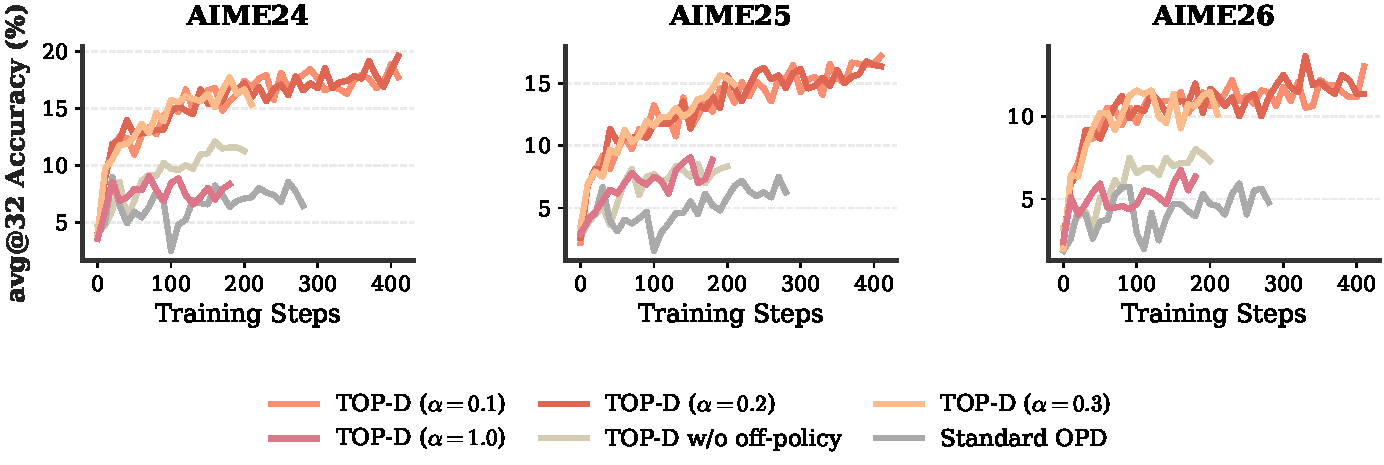
\includegraphics[scale=0.5]{ablation_curves.pdf}
	\caption{Learning curves for the ablation study on the Qwen3-1.7B-Base. We isolate the effects of the external proximal teacher ($\alpha=1.0$) and the internal trust region iterations (w/o off-policy).}
	\label{ablation curves}
\end{figure*}



\section{Conclusion}
In this paper, we introduce Trust Region Policy Distillation (TOP-D), a principled post-training paradigm resolving the optimization instability and sample inefficiency of standard On-Policy Distillation (OPD). Theoretically, TOP-D bounds gradient variance via an external proximal teacher and guarantees monotonic improvement with safe off-policy data reuse through internal trust region iterations. Empirically, it achieves massive performance gains on mathematical reasoning benchmarks, decisively outperforming standard OPD and competitive RLVR baselines across multiple model scales. By achieving these advancements without any additional computational overhead, TOP-D establishes a highly reliable, sample-efficient, and robust paradigm for aligning foundation models.




\bibliography{references}
\bibliographystyle{plainnat}






%%%%%%%%%%%%%%%%%%%%%%%%%%%%%%%%%%%%%%%%%%%%%%%%%%%%%%%%%%%%
\appendix

\newpage
\section{More Results}


\begin{table}[!h]
	\centering
	\renewcommand{\arraystretch}{1.1}
	\resizebox{\linewidth}{!}{
		\begin{tabular}{llc ccc ccc}
			\toprule
			\multirow{4}{*}[-0.8em]{\textbf{Student Model}} & \multirow{4}{*}[-0.8em]{\textbf{Paradigm}} & \multirow{4}{*}[-0.8em]{\textbf{Method}} & \multicolumn{6}{c}{\textbf{Teacher Model}} \\
			\cmidrule(lr){4-9}
			& & & \multicolumn{6}{c}{\textit{\textbf{Qwen3-30B-A3B-Instruct-2507}}} \\
			\cmidrule(lr){4-9}
			& & & \multicolumn{4}{c}{\textbf{avg@32}} & \multicolumn{2}{c}{\textbf{avg@8}} \\
			\cmidrule(lr){4-7} \cmidrule(lr){8-9}
			& & & \textbf{AIME24} & \textbf{AIME25} & \textbf{AIME26} & \textbf{AMC23} & \textbf{MATH-500} & \textbf{Olympiad} \\
			\midrule
			
			\multirow{5}{*}{\textit{\textbf{Qwen3-1.7B-Base}}} 
			& \textbf{Base} & - & 3.44 & 1.98 & 1.88 & 27.27 & 56.80 & 24.00 \\
			\cmidrule(l){2-9}
			& \multirow{2}{*}{\textbf{RLVR}} & GRPO & 10.52 & 7.19 & 4.69 & 35.55 & 54.73 & 18.47 \\
			& & DAPO & 12.29 & 11.56 & 8.54 & 37.50 & 61.88 & 26.63 \\
			\cmidrule(l){2-9}
			& \multirow{2}{*}{\textbf{Distillation}} & OPD & 8.96 & 7.50 & 5.94 & 45.70 & 71.13 & 35.83 \\
			& & \cellcolor{1}\textbf{TOP-D (Ours)} & \cellcolor{1}\textbf{20.31} {\color{2}\scriptsize\textbf{(+11.35)}} & \cellcolor{1}\textbf{17.71} {\color{2}\scriptsize\textbf{(+10.21)}} & \cellcolor{1}\textbf{13.75} {\color{2}\scriptsize\textbf{(+7.81)}} & \cellcolor{1}\textbf{54.38} {\color{2}\scriptsize\textbf{(+8.68)}} & \cellcolor{1}\textbf{77.33} {\color{2}\scriptsize\textbf{(+6.20)}} & \cellcolor{1}\textbf{43.06} {\color{2}\scriptsize\textbf{(+7.23)}} \\
			\bottomrule
		\end{tabular}
	}
	\caption{Performance comparison of the Qwen3-1.7B-Base across various mathematical benchmarks.}
\end{table}



\section*{Computational Resources}
All primary experiments, including the training of the TOP-D and the reproduction of baseline methods, were conducted on a high-performance computing cluster equipped with NVIDIA H200 GPUs. To accelerate the research iteration cycle, our standard distributed training setup utilized 4 compute nodes, with each node containing 8 H200 GPUs (amounting to 32 GPUs in total). However, we emphasize that our proposed method is highly resource-efficient and accessible. The entire TOP-D training pipeline and its reported results can be fully reproduced on a single standard 8-GPU node.





\section*{Limitations}
Although TOP-D establishes a highly reliable and sample-efficient paradigm for policy distillation, yielding massive improvements over existing baselines, our current validation is naturally bounded by computational budgets and time constraints. Specifically, our primary validations focus on student models up to the 8B parameter scale. Due to resource limitations, we have not yet investigated the scaling behavior of TOP-D on massive-scale foundation models (e.g., scaling the student model beyond 30B parameters). However, given the theoretically grounded variance-reduction properties of our proximal teacher and the guaranteed monotonic improvement from our trust region iterations, we are optimistic that the robust performance of TOP-D will seamlessly transfer to larger-scale regimes. 

Furthermore, our current empirical evaluations are constrained to a relatively short optimization window of only approximately 200 to 400 update steps (except for the RLVR baselines). Crucially, we have not observed any empirical signs of performance saturation within this timeframe. This strongly suggests that the impressive results reported in our main text are far from their upper bounds, leaving substantial room for further improvements with continued training. We leave the exploration of such extreme-scale distillation and extended training horizons as exciting avenues for future work.

\newpage
\section{Hyperparameters}\label{Hyperparameters}
\begin{table}[!h]
	\centering
	\renewcommand{\arraystretch}{1.2}
	\resizebox{1.0\linewidth}{!}{
		\begin{tabular}{l c c c c}
			\toprule
			\textbf{Hyperparameter} & \textbf{GRPO} \citep{shao2024deepseekmath} & \textbf{DAPO} \citep{yu2025dapo} & \textbf{OPD} \citep{lu2025onpolicydistillation} & \textbf{TOP-D (Ours)} \\
			\midrule
			
			\rowcolor{0}\multicolumn{5}{l}{\textit{\textbf{General}}} \\
			Max prompt length & 2048 & 2048 & 2048 & 2048 \\
			
			\midrule
			\rowcolor{0}\multicolumn{5}{l}{\textit{\textbf{Optimization}}} \\
			Global batch size & 512 & 512 & 512 & 512 \\
			Mini-batch size & 32 & 32 & 512 & 32 \\
			Mini-batches & 16 & 16 & 1 & 16 \\
			Group size & 8 & 8 & 8 & 8 \\
			Off-policy epoch & 1 & 1 & - & 1 \\
			Optimizer & AdamW & AdamW & AdamW & AdamW \\
			Learning rate & 1e-6 & 1e-6 & 1e-6 & 1e-6 \\
			Warmup steps & 10 & 10 & - & - \\
			
			\midrule
			\rowcolor{0}\multicolumn{5}{l}{\textit{\textbf{Sampling}}} \\
			Rollout max response length & 16384 & 16384 & 16384 & 16384 \\
			Rollout temperature & 1.0 & 1.0 & 1.0 & 1.0 \\
			Rollout top-$p$ & 1.0 & 1.0 & 1.0 & 1.0 \\
			Validation max response length & 16384 & 16384 & 16384 & 16384 \\
			Validation temperature & 1.0 & 1.0 & 1.0 & 1.0 \\
			Validation top-$p$ & 0.7 & 0.7 & 0.7 & 0.7 \\
			
			\midrule
			\rowcolor{0}\multicolumn{5}{l}{\textit{\textbf{Algorithm-specific}}} \\
			$\epsilon_{\mathrm{low}}$ & 0.2 & 0.2 & - & 0.2 \\
			$\epsilon_{\mathrm{high}}$ & 0.2 & 0.28 & - & 0.2 \\
			Interpolation $\alpha$ & - & - & - & 0.1 / 0.2 \\
			
			\bottomrule
		\end{tabular}
	}
	\caption{Detailed hyperparameters for different methods.}
	\label{hyperparameters}
\end{table}




\newpage
\section{Proofs}

\subsection{Proof of Theorem \ref{bounded variance}} \label{proof of bounded variance}
\textbf{Theorem \ref{bounded variance}.} \textit{
	Under Assumption \ref{assumption 1}, for any interpolation coefficient $\alpha\in(0,1)$, the variance of the TOP-D gradient estimator $\tilde{g}_k$ does not diverge across the entire probability space. Instead, it is strictly bounded by a uniform absolute limit:
	\begin{equation}
		\mathrm{Var}(\tilde{g}_k)\leq M^2\lvert\mathcal{V}\rvert\max\left\{\left(\log(1-\alpha)\right)^2, C^*\alpha\right\},
	\end{equation}
	where $C^*$ is a universal mathematical constant, and $\lvert\mathcal{V}\rvert$ denotes the size of the vocabulary $\mathcal{V}$.
}
\begin{proof}
	By the fundamental definition of variance, for any random vector $g$, $\mathrm{Var}(g)\leq\mathbb{E}\left[\lVert g\rVert^2\right]$. Thus, it suffices to establish a uniform upper bound for the gradient's second moment $\mathbb{E}\left[\lVert\tilde{g}_k\rVert^2\right]$.
	
	The TOP-D immediate reward is $\tilde{r}_k=\log\left(\alpha\rho_k+1-\alpha\right)$. Given a specific prompt $x$ and a generated prefix $y_{<k}$, we analyze the conditional expectation of the squared TOP-D reward $\tilde{r}_k^2$ over the finite vocabulary $\mathcal{V}$ at $k$-th token:
	\begin{equation}
		\mathbb{E}_{y_k \sim \pi_\theta(\cdot \mid x, y_{<k})}\left[\tilde{r}_k^2\right] = \sum_{y_k \in \mathcal{V}} \pi_\theta(y_k \mid x, y_{<k}) \left( \log\left(\alpha \frac{\pi^*(y_k \mid x, y_{<k})}{\pi_\theta(y_k \mid x, y_{<k})} + 1 - \alpha\right) \right)^2.
	\end{equation}
	For simplicity, let $p = \pi_\theta(y_k \mid x, y_{<k})$ and $q = \pi^*(y_k \mid x, y_{<k})$, where $p, q \in (0, 1)$. We define the objective term for each token in the summation as
	\begin{equation}
		h(p, q) = p \left( \log\left(\alpha \frac{q}{p} + 1 - \alpha\right) \right)^2.
	\end{equation}
	We seek to find the global supremum of $h(p, q)$ over the open domain $(p, q) \in (0, 1) \times (0, 1)$ by splitting it into two regions:
	
	\textbf{Case 1: The negative reward region $q < p$.}
	
	In this region, $\frac{q}{p} < 1$, so the inner logarithmic term satisfies $\alpha \frac{q}{p} + 1 - \alpha < 1$. Its infimum is approached as $q \to 0^+$, giving a strict lower bound of $1 - \alpha$. Therefore, $1 - \alpha < \alpha \frac{q}{p} + 1 - \alpha < 1$. The squared logarithm is bounded by
	\begin{equation}
		\left(\log\left(\alpha \frac{q}{p} + 1 - \alpha\right)\right)^2 < \left(\log(1 - \alpha)\right)^2.
	\end{equation}
	Since $p \in (0, 1)$, we directly bound the entire term:
	\begin{equation}
		h(p, q) < (\log(1 - \alpha))^2.
	\end{equation}
	
	\textbf{Case 2: The positive reward region $q \geq p$.}
	
	Here, $\frac{q}{p} \geq 1$. Since we strictly know $q < 1$, we can upper bound the ratio $\frac{q}{p} < \frac{1}{p}$. Because the function $(\log(\alpha x + 1 - \alpha))^2$ is monotonically increasing for $x \geq 1$, we can relax $h(p, q)$ into a univariate upper bounding function solely dependent on $p$:
	\begin{equation}
		h(p, q) < p \left( \log\left(\alpha \frac{1}{p} + 1 - \alpha\right) \right)^2.
	\end{equation}
	Furthermore, since $1 - \alpha > 0$ as $\alpha \in (0, 1)$, we can slightly loosen the inner term for algebraic simplicity without affecting its asymptotic behavior: $\frac{\alpha}{p} + 1 - \alpha < \frac{\alpha}{p} + 1$. Because the logarithm is monotonic, this substitution strictly bounds the function from above:
	\begin{equation}
		h(p, q) < p \left( \log\left(\alpha \frac{1}{p} + 1 - \alpha\right) \right)^2<p \left( \log\left(\frac{\alpha}{p} + 1\right) \right)^2.
	\end{equation}
	Next, let $u = \frac{1}{p}\in (1, \infty)$. We define the ultimate boundary function for this region:
	\begin{equation}
		f(u) = \frac{\left(\log(\alpha u + 1)\right)^2}{u}.
	\end{equation}
	To find the global maximum of $f(u)$ on $(1, \infty)$, we compute its derivative with respect to $u$:
	\begin{equation}
		f'(u) = \frac{2 \log(\alpha u + 1) \cdot \frac{\alpha}{\alpha u + 1} \cdot u - \left(\log(\alpha u + 1)\right)^2}{u^2}.
	\end{equation}
	Setting $f'(u) = 0$ identifies the stationary points. Since $u > 1$ and $\alpha \in (0, 1)$, the term $\log(\alpha u + 1) > 0$ and can be safely factored out. The condition simplifies to
	\begin{equation}
		\frac{2\alpha u}{\alpha u + 1} = \log(\alpha u + 1).
	\end{equation}
	We further introduce a variable substitution $t = \alpha u + 1$. Because $\alpha u > 0$, we have $t > 1$. Noting that $\alpha u = t - 1$, the condition transforms into a pure transcendental equation independent of $\alpha$:
	\begin{equation}
		2\left(1-\frac{1}{t}\right) = \log t \implies \log t - 2\left(1 - \frac{1}{t}\right) = 0.
	\end{equation}
	Let $w(t) = \log t - 2\left(1 - \frac{1}{t}\right)$. We analyze its roots for $t > 1$:
	\begin{enumerate}
		\item The derivative is $w'(t) = \frac{1}{t} - \frac{2}{t^2} = \frac{t - 2}{t^2}$.
		\item For $t \in (1, 2)$, $w'(t) < 0$, meaning $w(t)$ strictly decreases. Since $\lim_{t \to 1^+} w(t) = 0$, $w(t) < 0$ for all $t \in (1, 2)$.
		\item For $t > 2$, $w'(t) > 0$, meaning $w(t)$ strictly increases.
		\item Since $w(2)=\log2-1 < 0$ and $w(e^2)=\frac{2}{e^2}>0$, by the Intermediate Value Theorem, there exists exactly one unique root $t^*$ in the interval $(2, e^2)$.
	\end{enumerate}
	Since there is only one critical point, this unique stationary point corresponds to the global maximum of $f(u)$. The optimal point is $u^* = \frac{t^* - 1}{\alpha}$. Substituting $u^*$ back into $f(u)$ yields the closed-form analytical upper bound:
	\begin{equation}
		f(u)\leq f(u^*)=\frac{\left(\log t^*\right)^2}{t^* - 1}\cdot\alpha.
	\end{equation}
	Let $C^* = \frac{\left(\log t^*\right)^2}{t^* - 1}$. We conclude that for $q \geq p$, the term is strictly bounded by $h(p, q) \leq C^* \alpha$.
	
	In summary, the function $h(p, q)$ is uniformly bounded across the entire open domain $(0, 1) \times (0, 1)$ by an absolute limit:
	\begin{equation}
		\sup_{p, q \in (0,1)} h(p, q) \leq \max\left\{\left(\log(1-\alpha)\right)^2, C^*\alpha\right\}.
	\end{equation}
	
	Because the conditional expectation is a sum over a finite vocabulary of size $\lvert\mathcal{V}\rvert$, and each individual term is strictly bounded by $\max\left\{\left(\log(1-\alpha)\right)^2, C^*\alpha\right\}$, the conditional expectation itself is absolutely bounded regardless of the specific context $(x, y_{<k})$:
	\begin{equation}
		\begin{split}
			\mathbb{E}_{y_k \sim \pi_\theta(\cdot \mid x, y_{<k})}\left[\tilde{r}_k^2\right] &= \sum_{y_k \in \mathcal{V}} \pi_\theta(y_k \mid x, y_{<k}) \left( \log\left(\alpha \frac{\pi^*(y_k \mid x, y_{<k})}{\pi_\theta(y_k \mid x, y_{<k})} + 1 - \alpha\right) \right)^2\\
			&= \sum_{y_k \in \mathcal{V}} h(p, q) \leq\lvert\mathcal{V}\rvert\max\left\{\left(\log(1-\alpha)\right)^2, C^*\alpha\right\}. \\
		\end{split}
	\end{equation}
	Now, we move to the TOP-D gradient estimator $\tilde{g}_k = \nabla_\theta \log \pi_\theta(y_k \mid x, y_{<k}) \cdot \tilde{r}_k$. According to Assumption \ref{assumption 1}, we have
	\begin{equation}
		\lVert\tilde{g}_k\rVert^2 \leq \lVert\nabla_\theta \log \pi_\theta(y_k \mid x, y_{<k})\rVert^2 \cdot \tilde{r}_k^2 \leq M^2 \tilde{r}_k^2.
	\end{equation}
	Taking the total expectation over the prompt distribution $x \sim \mathcal{D}_x$, the autoregressive prefix trajectories $y_{<k} \sim \pi_\theta(\cdot \mid x)$, and the current token $y_k \sim \pi_\theta(\cdot \mid x, y_{<k})$, we apply the law of iterated expectations:
	\begin{equation}
		\begin{split}
			\mathbb{E}[\lVert\tilde{g}_k\rVert^2] &= \mathbb{E}_{x \sim \mathcal{D}_x, y_{<k} \sim \pi_\theta(\cdot \mid x)} \left[ \mathbb{E}_{y_k \sim \pi_\theta(\cdot \mid x, y_{<k})} \left[ \lVert\tilde{g}_k\rVert^2 \right] \right] \\
			&\leq\mathbb{E}_{x \sim \mathcal{D}_x, y_{<k} \sim \pi_\theta(\cdot \mid x)} \left[ M^2 \mathbb{E}_{y_k \sim \pi_\theta(\cdot \mid x, y_{<k})}\left[\tilde{r}_k^2\right]\right]\\
			&\leq\mathbb{E}_{x \sim \mathcal{D}_x, y_{<k} \sim \pi_\theta(\cdot \mid x)} \left[ M^2 \lvert\mathcal{V}\rvert\max\left\{\left(\log(1-\alpha)\right)^2, C^*\alpha\right\}\right]\\
			&=M^2\lvert\mathcal{V}\rvert\max\left\{\left(\log(1-\alpha)\right)^2, C^*\alpha\right\}.\\
		\end{split}
	\end{equation}
	Finally, returning to our variance inequality established at the beginning of the proof:
	\begin{equation}
		\mathrm{Var}(\tilde{g}_k) \leq \mathbb{E}\left[\lVert\tilde{g}_k\rVert^2\right] \leq M^2\lvert\mathcal{V}\rvert\max\left\{\left(\log(1-\alpha)\right)^2, C^*\alpha\right\}.
	\end{equation}
	Since $M$, $\lvert\mathcal{V}\rvert$, $\alpha$, and $C^*$ are all finite, the exact gradient variance is absolutely bounded. The proof is now complete.
\end{proof}






\subsection{Proof of Theorem \ref{convergence}} \label{proof of convergence}
\textbf{Theorem \ref{convergence}.} \textit{
	For any initial student policy $\pi_0\in\Pi$, consider the iterative update process $\pi_{k+1}=\mathcal{T}(\pi_k)+\epsilon_k$, where $\epsilon_k$ accounts for the practical optimization error (e.g., function approximation and optimization noise) at the $k$-th global step, where $k\geq0$. Then, the following bound holds:
	\begin{equation}
		d(\pi_{k+1},\pi^*)\leq(1-\alpha)^{k+1}d(\pi_0,\pi^*)+\sum_{i=0}^{k}(1-\alpha)^{k-i}\lVert\epsilon_i\rVert_1.
	\end{equation}
	Furthermore, assuming the optimization process eventually stabilizes such that the asymptotic error is bounded by $\limsup_{k\rightarrow \infty}\lVert\epsilon_{k}\rVert_1\leq \epsilon_{\infty}$, we have
	\begin{equation}
		\limsup_{k \rightarrow \infty} d(\pi_{k+1}, \pi^*) \leq \frac{\epsilon_{\infty}}{\alpha}.
	\end{equation}
}
\begin{proof}
	We aim to bound the expected $L_1$ distance between the student policy $\pi_{k+1}$ and the optimal target teacher policy $\pi^*$.
	
	\textbf{Step 1: Establishing the single-step recurrence relation.}
	
	According to the iterative update process defined in the theorem, for any global step $k \geq 0$, the updated policy is given by
	\begin{equation}
		\pi_{k+1} = \mathcal{T}(\pi_k) + \epsilon_k,
	\end{equation}
	where $\mathcal{T}:\Pi\to\Pi$ is the \textit{proximal teacher operator} defined in \eqref{proximal teacher operator}. By utilizing the triangle inequality of the expected $L_1$ distance metric $d(\cdot, \cdot)$, we decouple the distance between the updated policy $\pi_{k+1}$ and the target policy $\pi^*$ into two components:
	\begin{equation}\label{triangle inequality}
		d(\pi_{k+1}, \pi^*) \leq d(\mathcal{T}(\pi_k), \pi^*) + d(\pi_{k+1}, \mathcal{T}(\pi_k)).
	\end{equation}
	We analyze the second term on the right-hand side first. As defined in the main text, the proximal teacher is explicitly given by $\tilde{\pi}_k^*=\mathcal{T}(\pi_k)=\alpha\pi^*+(1-\alpha)\pi_k$. Therefore, the distance between the updated policy $\pi_{k+1}$ and the proximal teacher $\mathcal{T}(\pi_k)$ precisely corresponds to the expected $L_1$ norm of the optimization error at step $k$:
	\begin{equation}
		d(\pi_{k+1}, \mathcal{T}(\pi_k)) = d(\pi_{k+1}, \tilde{\pi}_k^*) = \lVert\epsilon_k\rVert_1.
	\end{equation}
	For the first term, we substitute the explicit definition of the proximal operator $\mathcal{T}(\pi_k)$. Utilizing the absolute homogeneity and linearity of the expected $L_1$ norm over $\mathcal{D}_x$, we obtain
	\begin{equation}
		\begin{split}
			d(\mathcal{T}(\pi_k), \pi^*)&=\mathbb{E}_{x\sim\mathcal{D}_x}\left[\lVert\alpha\pi^*(\cdot\mid x)+(1-\alpha)\pi_k(\cdot\mid x)-\pi^*(\cdot\mid x)\rVert_1\right]\\
			&=(1-\alpha)\mathbb{E}_{x\sim\mathcal{D}_x}\left[\lVert\pi_k(\cdot\mid x)-\pi^*(\cdot\mid x)\rVert_1\right]\\
			&=(1-\alpha)d(\pi_k,\pi^*).
		\end{split}
	\end{equation}
	Substituting both decoupled terms back into the triangle inequality \eqref{triangle inequality}, we establish the strict single-step recurrence relation for any step:
	\begin{equation}
		d(\pi_{k+1}, \pi^*) \leq(1-\alpha)d(\pi_k,\pi^*)+\lVert\epsilon_k\rVert_1.
	\end{equation}
	
	\textbf{Step 2: Forward unrolling of the recurrence relation.}
	
	To derive the explicit global bound for step $k+1$, we recursively unroll this single-step bound forward, starting from the initial step $k=0$.
	
	For $k=0$, the single-step recurrence gives
	\begin{equation}
		d(\pi_{1}, \pi^*) \leq(1-\alpha)d(\pi_0,\pi^*)+\lVert\epsilon_0\rVert_1.
	\end{equation}
	
	For $k=1$, we apply the recurrence and substitute the previously established bound for $d(\pi_{1}, \pi^*)$:
	\begin{equation}
		\begin{split}
			d(\pi_{2}, \pi^*) &\leq(1-\alpha)d(\pi_1,\pi^*)+\lVert\epsilon_1\rVert_1\\
			&\leq(1-\alpha)^2d(\pi_0,\pi^*)+(1-\alpha)\lVert\epsilon_0\rVert_1+\lVert\epsilon_1\rVert_1.
		\end{split}
	\end{equation}
	
	For $k=2$, we repeat the process by substituting the bound for $d(\pi_{2}, \pi^*)$:
	\begin{equation}
		\begin{split}
			d(\pi_{3}, \pi^*) &\leq(1-\alpha)d(\pi_2,\pi^*)+\lVert\epsilon_2\rVert_1\\
			&\leq(1-\alpha)^3d(\pi_0,\pi^*)+(1-\alpha)^2\lVert\epsilon_0\rVert_1+(1-\alpha)\lVert\epsilon_1\rVert_1+\lVert\epsilon_2\rVert_1.
		\end{split}
	\end{equation}
	Through rigorous algebraic expansion by repeating this substitution multiple times, a clear geometric pattern emerges. Accumulating these terms yields the closed-form finite-step global bound:
	\begin{equation}
		d(\pi_{k+1}, \pi^*)\leq(1-\alpha)^{k+1}d(\pi_0,\pi^*)+\sum_{i=0}^{k}(1-\alpha)^{k-i}\lVert\epsilon_i\rVert_1.
	\end{equation}
	
	\textbf{Step 3: Deriving the asymptotic convergence bound.}
	
	To determine the asymptotic behavior, we apply the limit supremum ($\limsup_{k \rightarrow \infty}$) to both sides of the inequality:
	\begin{equation}
		\limsup_{k \rightarrow \infty}d(\pi_{k+1}, \pi^*)\leq\limsup_{k \rightarrow \infty}\left\{(1-\alpha)^{k+1}d(\pi_0,\pi^*)+\sum_{i=0}^{k}(1-\alpha)^{k-i}\lVert\epsilon_i\rVert_1\right\}.
	\end{equation}
	First, the interpolation coefficient satisfies $\alpha \in (0, 1)$. Consequently, the term associated with the initial distance decays exponentially to zero:
	\begin{equation}
		\limsup_{k \rightarrow \infty}(1-\alpha)^{k+1}d(\pi_0,\pi^*)=0.
	\end{equation}
	Next, we analyze the accumulated error summation term. We are given the assumption that the asymptotic optimization error is bounded, i.e., $\limsup_{k\rightarrow \infty}\lVert\epsilon_{k}\rVert_1\leq \epsilon_{\infty}$. By the mathematical definition of the limit supremum, for any arbitrarily small constant $\delta > 0$, there exists a sufficiently large integer $N > 0$ such that for all $i \geq N$, the condition $\lVert\epsilon_i\rVert_1 \leq \epsilon_{\infty} + \delta$ strictly holds.
	
	Let $k\to\infty$, we now split the summation into two parts at this critical index $N$:
	\begin{equation}
		\sum_{i=0}^{k}(1-\alpha)^{k-i}\lVert\epsilon_i\rVert_1=\sum_{i=0}^{N-1}(1-\alpha)^{k-i}\lVert\epsilon_i\rVert_1+\sum_{i=N}^{k}(1-\alpha)^{k-i}\lVert\epsilon_i\rVert_1.
	\end{equation}
	As $k \to \infty$, the first term vanishes to zero. For the second term, we safely substitute the uniform bound $\lVert\epsilon_i\rVert_1 \leq \epsilon_{\infty} + \delta$ for all terms where $i \geq N$:
	\begin{equation}
		\sum_{i=N}^{k}(1-\alpha)^{k-i}\lVert\epsilon_i\rVert_1\leq(\epsilon_{\infty}+\delta)\sum_{i=N}^{k}(1-\alpha)^{k-i}.
	\end{equation}
	We introduce a change of variable by letting $j = k - i$. When $i = k$, $j=0$. When $i=N$, $j = k - N$. This transforms the summation into a standard geometric series:
	\begin{equation}
		(\epsilon_{\infty}+\delta)\sum_{i=N}^{k}(1-\alpha)^{k-i}=(\epsilon_{\infty}+\delta)\sum_{j=0}^{k-N}(1-\alpha)^{j}.
	\end{equation}
	Now we have
	\begin{equation}
		\limsup_{k\rightarrow \infty}\sum_{i=N}^{k}(1-\alpha)^{k-i}\lVert\epsilon_i\rVert_1\leq\limsup_{k\rightarrow \infty}(\epsilon_{\infty}+\delta)\sum_{j=0}^{k-N}(1-\alpha)^{j}=(\epsilon_{\infty}+\delta)\sum_{j=0}^{\infty}(1-\alpha)^{j}=\frac{\epsilon_{\infty}+\delta}{\alpha}.
	\end{equation}
	Because the choice of $\delta > 0$ is arbitrary and can be chosen to be infinitesimally small ($\delta \to 0$), the limit supremum of the entire sequence is strictly bounded by $\epsilon_{\infty}/\alpha$. Combining this bound with the vanishing first term, we have
	\begin{equation}
		\limsup_{k \rightarrow \infty}d(\pi_{k+1}, \pi^*)\leq\frac{\epsilon_{\infty}}{\alpha}.
	\end{equation}
	The proof is now complete.
\end{proof}





\subsection{Proof of Theorem \ref{performance lower bound}} \label{proof of performance lower bound}
\textbf{Theorem \ref{performance lower bound}.} \textit{
	Given Assumption \ref{assumption 2} and Definition \ref{normalized state distribution}, for any two policies, $\tilde{\pi}$ and $\pi$, the following bound holds:
	\begin{equation}
		\eta(\tilde{\pi})\geq\zeta_\pi(\tilde{\pi}) - 2\xi T_{\max}\ell_\pi\mathbb{E}_{s \sim d^{\pi}_{\mathrm{norm}}(\cdot)}\left[\mathcal{D}_{\mathrm{TV}}(\tilde{\pi}(\cdot \mid s),\pi(\cdot \mid s))\right],
	\end{equation}
	where $\zeta_\pi(\tilde{\pi})=\eta(\pi) + \ell_\pi\mathbb{E}_{s \sim d^\pi_{\mathrm{norm}}(\cdot), a \sim \tilde{\pi}(\cdot \mid s)} \left[ A^\pi(s, a) \right]$, and $\xi=\max_{s}\lvert\mathbb{E}_{a\sim\tilde{\pi}(\cdot\mid s)}\left[A^\pi(s,a)\right]\rvert$.
}
\begin{proof}
	To establish the monotonic improvement lower bound, we begin by bounding the absolute error between the true expected return $\eta(\tilde{\pi})$ and our constructed surrogate objective $\zeta_\pi(\tilde{\pi})$.
	
	First, we express the unnormalized performance difference:
	\begin{equation}
		\eta(\tilde{\pi}) = \eta(\pi)+\sum_{s \neq s_\bot} d^{\tilde{\pi}}(s) \sum_{a \in \mathcal{V}} \tilde{\pi}(a \mid s) A^\pi(s, a).
	\end{equation}
	$\zeta_\pi(\tilde{\pi})$ is anchored to the base policy's normalized state distribution. By applying Definition \ref{normalized state distribution}, where $d^\pi(s) = \ell_\pi d^\pi_{\mathrm{norm}}(s)$, we can unroll $\zeta_\pi(\tilde{\pi})$ back into the unnormalized measure space:
	\begin{equation}
		\zeta_\pi(\tilde{\pi}) = \eta(\pi) + \sum_{s \neq s_\bot} d^\pi(s) \sum_{a \in \mathcal{V}} \tilde{\pi}(a \mid s) A^\pi(s, a).
	\end{equation}
	We isolate the objective approximation error by subtracting $\zeta_\pi(\tilde{\pi})$ from $\eta(\tilde{\pi})$. By applying Hölder's Inequality, we decouple the global state distribution shift from the local expected advantage drift:
	\begin{equation}\label{decoupled objective approximation error}
		\lvert \eta(\tilde{\pi}) - \zeta_\pi(\tilde{\pi}) \rvert \leq \left( \sum_{s \neq s_\bot} \lvert d^{\tilde{\pi}}(s) - d^\pi(s) \rvert \right) \cdot \max_s \left\lvert \sum_{a \in \mathcal{V}} \tilde{\pi}(a \mid s) A^\pi(s, a) \right\rvert.
	\end{equation}
	The second decoupled term is precisely defined as our constant $\xi=\max_{s}\lvert\mathbb{E}_{a\sim\tilde{\pi}(\cdot\mid s)}\left[A^\pi(s,a)\right]\rvert$.
	
	Next, we rigorously bound the $L_1$ norm of the unnormalized global measure shift. Since the unnormalized measure is the sum of marginal state probabilities over time, we expand this across the maximum generation horizon $T_{\max}$ defined in Assumption \ref{assumption 2}, and apply the triangle inequality:
	\begin{equation}
		\sum_{s \neq s_\bot} \lvert d^{\tilde{\pi}}(s) - d^\pi(s) \rvert \leq \sum_{t=1}^{T_{\max}} \sum_{s \neq s_\bot} \lvert \mathbb{P}(s_t = s \mid \tilde{\pi}) - \mathbb{P}(s_t = s \mid \pi) \rvert.
	\end{equation}
	At the first generation step $t=1$, the initial state $s_1$ is strictly defined by the input prompt $x \sim \mathcal{D}_x$ and the special initial token $y_0$. Because this initial distribution is completely independent of the policy, the marginal probability distance is exactly zero:
	\begin{equation}
		\sum_{s \neq s_\bot} \lvert \mathbb{P}(s_1 = s \mid \tilde{\pi}) - \mathbb{P}(s_1 = s \mid \pi) \rvert = 0.
	\end{equation}
	For any subsequent generation step $t > 1$, we construct a telescoping sum to bound the difference in marginal probabilities. Let $\mathbb{P}_i$ denote a \textit{hybrid trajectory distribution} where the first $i$ steps are generated by the behavior policy $\pi$, and the remaining steps from $i+1$ to $t-1$ are generated by the target policy $\tilde{\pi}$. Note that $\mathbb{P}_{t-1}$ represents full generation under $\pi$, and $\mathbb{P}_0$ represents full generation under $\tilde{\pi}$. The telescoping sum bridging these two extreme distributions is given by
	\begin{equation}
		\mathbb{P}(s_t = s \mid \tilde{\pi}) - \mathbb{P}(s_t = s \mid \pi)=\mathbb{P}_0-\mathbb{P}_{t-1}=-\sum_{i=1}^{t-1} \left( \mathbb{P}_i(s_t = s) - \mathbb{P}_{i-1}(s_t = s) \right).
	\end{equation}
	Taking the absolute value and applying the triangle inequality yields
	\begin{equation}
		\sum_{s \neq s_\bot}\lvert\mathbb{P}(s_t = s \mid \tilde{\pi}) - \mathbb{P}(s_t = s \mid \pi)\rvert\leq\sum_{s \neq s_\bot}\sum_{i=1}^{t-1} \lvert\mathbb{P}_i(s_t = s) - \mathbb{P}_{i-1}(s_t = s)\rvert.
	\end{equation}
	Observe that the adjacent hybrid distributions $\mathbb{P}_i$ and $\mathbb{P}_{i-1}$ share the identical generation history up to step $i-1$ (governed by $\pi$) and share the identical rollout strategy from step $i+1$ onward (governed by $\tilde{\pi}$). They diverge only at the specific decision step $i$.
	
	In our autoregressive generation framework, the environmental transitions are purely deterministic (appending the generated token to the prefix). Consequently, summing over all possible future states $s_t$ effectively marginalizes them out, collapsing the trajectory distance precisely to the expected $L_1$ divergence of the action distributions at the singular branching step $i$:
	\begin{equation}
		\sum_{s \neq s_\bot}\lvert\mathbb{P}_i(s_t = s) - \mathbb{P}_{i-1}(s_t = s)\rvert \leq \mathbb{E}_{s_i \sim \mathbb{P}(s_i \mid \pi)}\left[ \lVert\tilde{\pi}(\cdot \mid s_i) - \pi(\cdot \mid s_i)\rVert_1 \right].
	\end{equation}
	Substituting this into our bound and summing over the entire telescoping sequence from $i=1$ to $t-1$, we obtain the marginal probability distance for a specific step $t$:
	\begin{equation}
		\sum_{s \neq s_\bot}\lvert\mathbb{P}(s_t = s \mid \tilde{\pi}) - \mathbb{P}(s_t = s \mid \pi)\rvert \leq 2\sum_{i=1}^{t-1} \mathbb{E}_{s_i \sim \mathbb{P}(s_i \mid \pi)}\left[\mathcal{D}_{\mathrm{TV}}(\tilde{\pi}(\cdot \mid s_i), \pi(\cdot \mid s_i))\right].
	\end{equation}
	As established earlier, the initial state distribution at $t=1$ is strictly fixed by the prompt and the special initial token, yielding zero divergence. Therefore, we sum this temporal bound over the valid response steps from $t=2$ to the maximum generation horizon $T_{\max}$ to measure the global shift:
	\begin{equation}
		\sum_{s \neq s_\bot} \lvert d^{\tilde{\pi}}(s) - d^\pi(s) \rvert \leq 2\sum_{t=2}^{T_{\max}}\sum_{i=1}^{t-1} \mathbb{E}_{s_i \sim \mathbb{P}(s_i \mid \pi)}\left[\mathcal{D}_{\mathrm{TV}}(\tilde{\pi}(\cdot \mid s_i), \pi(\cdot \mid s_i))\right].
	\end{equation}
	To efficiently decouple this complex temporal accumulation, we rearrange the nested summations. By exchanging the order of summation between the time steps, we observe that the expected divergence at any step $i$ is repeatedly accumulated exactly $(T_{\max} - i)$ times:
	\begin{equation}
		\begin{split}
			&\sum_{t=2}^{T_{\max}}\sum_{i=1}^{t-1} \mathbb{E}_{s_i \sim \mathbb{P}(s_i \mid \pi)}\left[\mathcal{D}_{\mathrm{TV}}(\tilde{\pi}(\cdot \mid s_i), \pi(\cdot \mid s_i))\right]\\ =& \sum_{i=1}^{T_{\max}-1} (T_{\max} - i) \mathbb{E}_{s_i \sim \mathbb{P}(s_i \mid \pi)}\left[\mathcal{D}_{\mathrm{TV}}(\tilde{\pi}(\cdot \mid s_i), \pi(\cdot \mid s_i))\right]\\
			\leq& T_{\max} \sum_{i=1}^{T_{\max}} \sum_{s \neq s_\bot} \mathbb{P}(s_i = s \mid \pi) \mathcal{D}_{\mathrm{TV}}(\tilde{\pi}(\cdot \mid s), \pi(\cdot \mid s)).\\
			=&T_{\max} \sum_{s \neq s_\bot} \mathcal{D}_{\mathrm{TV}}(\tilde{\pi}(\cdot \mid s), \pi(\cdot \mid s)) \left( \sum_{i=1}^{T_{\max}} \mathbb{P}(s_i = s \mid \pi) \right).\\
		\end{split}
	\end{equation}
	Here, we relax this sum by bounding the varying coefficient $(T_{\max} - i)$ with the uniform maximum horizon $T_{\max}$ and expand the expectation into a summation over specific states.
	
	Since the unnormalized state measure $d^\pi(s)$ intrinsically aggregates the expected distribution across all steps by definition, i.e., $d^\pi(s) = \sum_{t=1}^{\infty}\mathbb{P}(s_t = s \mid \pi) \geq \sum_{i=1}^{T_{\max}} \mathbb{P}(s_i = s \mid \pi)$, we can concisely upper-bound the relaxed sequence, so
	\begin{equation}
		\sum_{s \neq s_\bot} \lvert d^{\tilde{\pi}}(s) - d^\pi(s) \rvert \leq 2T_{\max} \sum_{s \neq s_\bot} d^\pi(s)\mathcal{D}_{\mathrm{TV}}(\tilde{\pi}(\cdot \mid s), \pi(\cdot \mid s)).
	\end{equation}
	Recalling Definition \ref{normalized state distribution}, we substitute the unnormalized measure with $d^\pi(s) = \ell_\pi d^\pi_{\mathrm{norm}}(s)$, gracefully transforming the summation into a formal expectation over the normalized state distribution:
	\begin{equation}
		\sum_{s \neq s_\bot} \lvert d^{\tilde{\pi}}(s) - d^\pi(s) \rvert \leq 2T_{\max}\ell_\pi\mathbb{E}_{s \sim d^{\pi}_{\mathrm{norm}}(\cdot)}\left[\mathcal{D}_{\mathrm{TV}}(\tilde{\pi}(\cdot \mid s),\pi(\cdot \mid s))\right].
	\end{equation}
	Finally, substituting this global measure shift bound back into our decoupled objective approximation error \eqref{decoupled objective approximation error}, we obtain the absolute bound for the objective difference:
	\begin{equation}
		\lvert \eta(\tilde{\pi}) - \zeta_\pi(\tilde{\pi}) \rvert \leq 2\xi T_{\max}\ell_\pi\mathbb{E}_{s \sim d^{\pi}_{\mathrm{norm}}(\cdot)}\left[\mathcal{D}_{\mathrm{TV}}(\tilde{\pi}(\cdot \mid s),\pi(\cdot \mid s))\right],
	\end{equation}
	which implies that
	\begin{equation}
		\eta(\tilde{\pi})\geq\zeta_\pi(\tilde{\pi}) - 2\xi T_{\max}\ell_\pi\mathbb{E}_{s \sim d^{\pi}_{\mathrm{norm}}(\cdot)}\left[\mathcal{D}_{\mathrm{TV}}(\tilde{\pi}(\cdot \mid s),\pi(\cdot \mid s))\right].
	\end{equation}
	The proof is now complete.
\end{proof}



%%%%%%%%%%%%%%%%%%%%%%%%%%%%%%%%%%%%%%%%%%%%%%%%%%%%%%%%%%%%




\end{document}